\documentclass{beamer}

\usepackage{graphics}
\usepackage{graphicx}
\usepackage{amsmath,amssymb,amsthm}
%\usepackage{subeqnarray}
%\usepackage{easybmat}
%\usepackage{subfigure}



%\usepackage{HA-prosper}
%\usepackage[dvips,letterpaper]{geometry}


\def\R{\mathcal{R}}
\def\D{\mathcal{D}}
\def\C{\mathcal{C}}
\def\IC{\mathbb{C}}
\def\IN{\mathbb{N}}
\def\IR{\mathbb{R}}
\def\Rzero{\mathcal{R}_0}
\def\diag{\textrm{diag}}
\def\tr{\textrm{tr}}
\def\det{\textrm{det}}
\def\sgn{\textrm{sgn}}
\def\imply{$\Rightarrow$}
\def\dbint{\int\!\!\!\int}
\def\dbintb{\mathop{\int\!\!\!\!\int}}
\def\tpint{\int\!\!\!\int\!\!\!\int}

\newtheorem{proposition}{Proposition}

\setbeamertemplate{navigation symbols}{}
\setbeamertemplate{footline}
{%
\quad\insertsection\hfill p. \insertpagenumber\quad\mbox{}\vskip2pt
}


\begin{document}
%\maketitle
\frame{\frametitle{A gentle introduction to Matlab}
The ``Mat'' in Matlab does not stand for ``mathematics'', but for ``matrix''..
\vskip1cm
$\Rightarrow$ all objects in matlab are matrices of some sort! Keep this in mind when using it.
\vskip1cm
Matlab is a high level \emph{interpreted} programming language: 
\begin{itemize}
\item a matlab program is typically a set of instructions that are evaluated iteratively;
\item most of the work can be done directly from the command line.
\end{itemize}
}

\section{Computing iterates}

\frame[containsverbatim]{\frametitle{Defining a function}
We want to plot the iterates of some function $f$. First, we define the function.
\begin{verbatim}
>> f=inline('r.*x.*(1-x)','x','r')

f =

     Inline function:
     f(x,r) = r.*x.*(1-x)
\end{verbatim}
This defines a function (here, with two arguments, $x$ and $r$), that can then be used:
\begin{verbatim}
>> f(0.2,3.2)

ans =

    0.5120
\end{verbatim}
}

\frame[containsverbatim]{\frametitle{``;'' hides the result on the command line}
Remark that
\begin{verbatim}
>> f(0.2,3.2)

ans =

    0.5120
\end{verbatim}
but
\begin{verbatim}
>> f(0.2,3.2);
\end{verbatim}
produces no output.
}

\frame[containsverbatim]{\frametitle{Creating a vector}
To create a vector, use the command
\[
x=\textrm{first entry}:\textrm{step}:\textrm{last entry},
\]
or, if entries are a subset of the integers,
\[
x=\textrm{first entry}:\textrm{last entry}.
\]
For example, we want to plot the iterates of the logistic map, so
\begin{verbatim}
x=0:0.01:1;
\end{verbatim}
Note the ``;'': otherwise, we get the full 101 elements vector displayed.
}

\frame[containsverbatim]{\frametitle{What is the size of .. ?}
As mentioned, in matlab everything is a matrix. For matrix operations, size is important, and it is frequent to make mistakes. To check, {\tt whos} and {\tt size}. {\tt whos} gives a lot of information.
\begin{verbatim}
>> whos x
  Name      Size                 Bytes  Class

  x         1x101                  808  double array
Grand total is 101 elements using 808 bytes
\end{verbatim}
Various variables can be listed on the line after {\tt whos}:
\begin{verbatim}
>> whos x k
  Name      Size                  Bytes  Class

  k         1x1                       8  double array
  x         1x101                   808  double array
Grand total is 102 elements using 816 bytes
\end{verbatim}
}

\frame[containsverbatim]{\frametitle{\tt size}
{\tt size}, on the other hand, is ``attributable''. It can be used like this
\begin{verbatim}
>> size(x)

ans =
     1   101
\end{verbatim}
but also like this, since the result is a vector
\begin{verbatim}
>> [r,c]=size(x)

r =
     1

c =
   101
\end{verbatim}
in which case, $r$ and $c$ take the values of the numbers of rows and columns, respectively.
}


\frame[containsverbatim]{\frametitle{Vectorized functions versus nonvectorized functions}
Recall that we wrote
\begin{verbatim}
>> f=inline('r.*x.*(1-x)','x','r')
\end{verbatim}
that is, every multiplication sign took the form \verb!.*! instead of \verb!*!. Here, this is needed: we want to use the \emph{vectorized} form of the function, and be able to pass to $f$ a vector instead of a single value. The \verb!.*! form means that the operation is applied to every entry in the vector/matrix. Same exists for \verb!/! and \verb!^!. Can also use the function {\tt vectorize}.
\vskip0.5cm
The result of using this vectorized form is that $f$ will be applied to every entry of $x$, and will produce a vector.
\vskip0.5cm
Vectorized operations have been optimized in matlab, and are extremely fast. When possible, they should be used instead of loops.
}

\frame[containsverbatim]{\frametitle{Vectorized vs nonvectorized}
Define
\begin{verbatim}
>> f=inline('r.*x.*(1-x)','x','r')
>> g=inline('r*x*(1-x)','x','r')
\end{verbatim}
and for simplicity, consider the vector
\begin{verbatim}
>> x=[1,2];
\end{verbatim}
Then
\begin{verbatim}
>> f(x,3.5)
   g(x,3.5)
ans =
     0    -7

??? Error using ==> inlineeval
Error in inline expression ==> r*x*(1-x)
??? Error using ==> mtimes
Inner matrix dimensions must agree.
\end{verbatim}
}

\frame[containsverbatim]{\frametitle{Plotting}
Basic plotting is very easy. The format is
\begin{verbatim}
plot(x_axis,y_value)
\end{verbatim}
so, for example (with $f$ as defined above),
\begin{verbatim}
plot(x,f(x,3.4))
\end{verbatim}
(here, ``;'' or not does not matter, as the figure appears in a new window and all that ``;'' changes is the output in the command window).
}

\frame{
\begin{center}
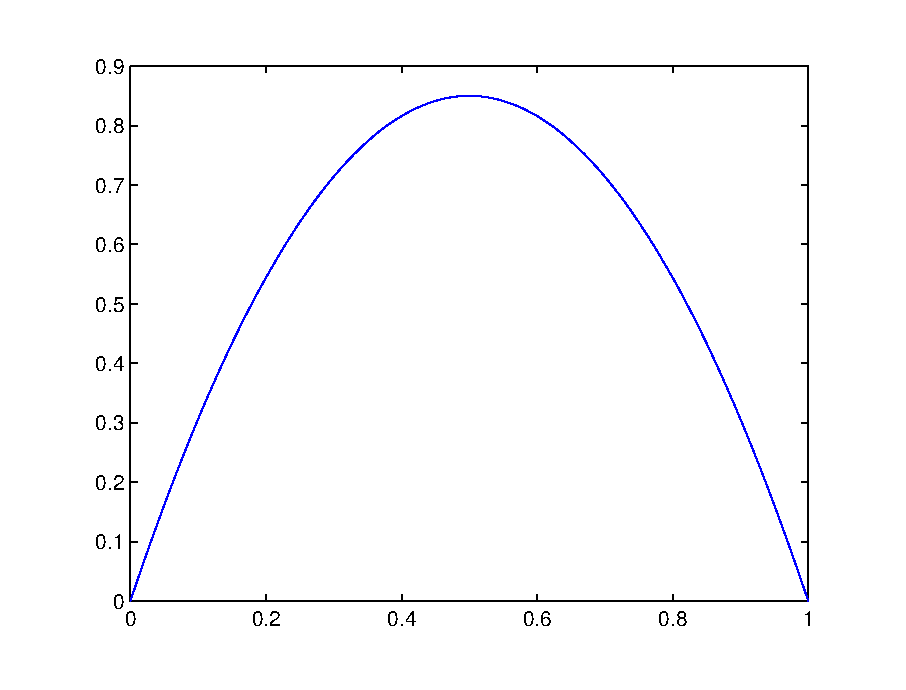
\includegraphics[width=\textwidth]{plot_iterates_1}
\end{center}
}


\frame[containsverbatim]{\frametitle{Making things a bit more fancy}
This is a very basic plot. 
\begin{itemize}
\item We could want to plot more than one object (for example, the line $y=x$ would be nice)..
\begin{verbatim}
plot(x,x,x,f(x,3.4));
\end{verbatim}
Ordering is by pairs: $x_1,f_1(x_1),x_2,f_2(x_2)$. Two elements in a pair {\bf must have} the same number of columns. Different pairs {\bf can have} different numbers of columns. Each element in a given pair can be a point, a vector, a matrix.
\item We could want to label the axes..
\begin{verbatim}
xlabel('x');
ylabel('f(x)');
\end{verbatim}
\end{itemize}
}

\frame{
\begin{center}
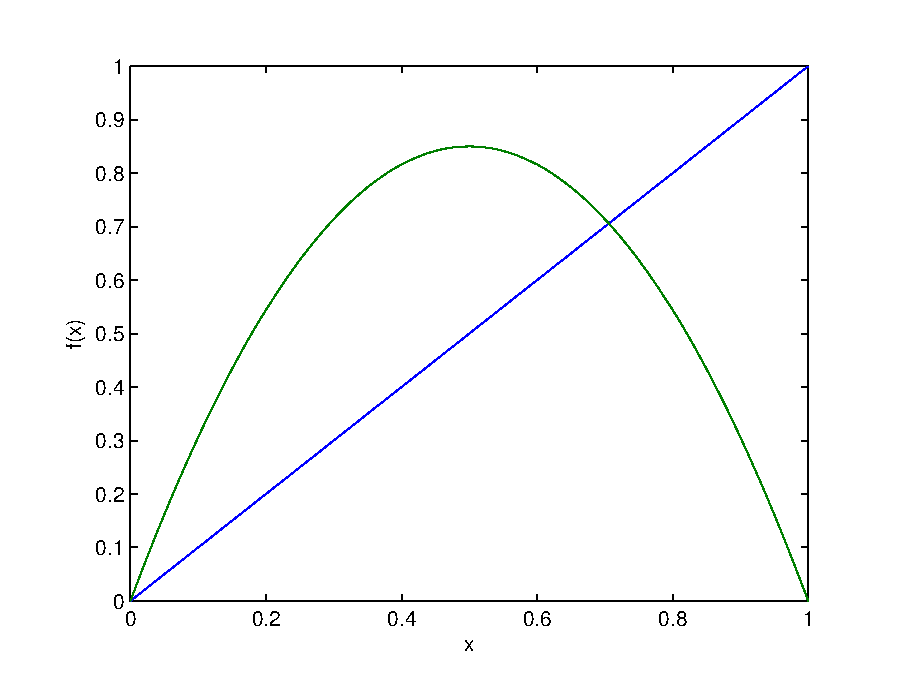
\includegraphics[width=\textwidth]{plot_iterates_2}
\end{center}
}

\frame[containsverbatim]{\frametitle{Computing several iterates}
For the moment, we only have $f(x)$. We want $f^n(x)$, for a given $n$. Several ways.
\begin{itemize}
\item Taking for example $r=3.5$, use
\begin{verbatim}
f(f(x,3.5),3.5)
\end{verbatim}
\item The downside to this method is that matlab does not allow to formally define $f^n$, so tricks have to be used for larger values of $n$, for example, produce a string containing the command 
\begin{verbatim}
f(f(f(f(f(x,3.5),3.5),3.5),3.5),3.5)
\end{verbatim}
and evaluate it. Complicated..
\item Another method consists in using the result found at the previous step to evaluate the next. We do that..
\end{itemize}
}


\frame[containsverbatim]{\frametitle{Automatic resizing of vectors and matrices}
We are going to use a very nice feature of matlab: adding elements to a vector, or rows/columns to a matrix, is automatic. Suppose for example that we had defined $x$ as
\begin{verbatim}
x=0:0.01:0.5;
\end{verbatim}
Then 
\begin{verbatim}
x=[x,0.51:0.01:1];
\end{verbatim}
would produce the vector $x$ as we had earlier.
}

\frame[containsverbatim]{\frametitle{}
{\bf Be careful!} Note that the command was
\begin{verbatim}
x=[x,0.51:0.01:1];
\end{verbatim}
that is, the old and new entries were separated by a ``,''. This is \emph{horizontal concatenation}. The command with a ``;'' tries to add a new row. In our case, we get
\begin{verbatim}
>> z=[z;0.51:0.01:1]
??? Error using ==> vertcat
All rows in the bracketed expression must have the same 
number of columns.
\end{verbatim}
because we are trying to add a row of 50 elements to a row of 51 elements. But
\begin{verbatim}
>> z=[z;0.51:0.01:1.01]
\end{verbatim}
works, and gives a $2\times 51$ matrix.
}

\frame[containsverbatim]{
Here, we are going to use the latter form of the command, and add each successive iterate to a solution matrix $M$.

First, define an empty matrix,
\begin{verbatim}
M=[];
\end{verbatim}
Then we need to loop from 1 to $n$, where $n$ is the iterate that we want. 
}

\frame[containsverbatim]{\frametitle{Loops}
The command uses the same type of syntax as the creation of a vector: to loop from $4$ to $12$ by steps of 1,
\begin{verbatim}
for i=4:12,
   command(s) to be repeated, maybe using the value i
end;
\end{verbatim}
whereas to loop by non-unit or non-integer steps, say from 4 to 12 by steps of 1.35,
\begin{verbatim}
for i=4:1.35:12,
   command(s) to be repeated, maybe using the value i
end;
\end{verbatim}
Note that in that case, the last $i$ is equal to $10.75$, not $12$, since $10.75+1.35=12.1>12$. The same is true when using non-unit steps to create vectors.
}

\frame{\frametitle{Accessing matrix elements}
Suppose that $M$ is an $m\times n$-matrix. Then
\begin{itemize}
\item {\tt M(i,j)} is the element on the $i$th row and $j$th column.
\item {\tt M(i,:)} is the $i$th row.
\item {\tt M(:,j)} is the $j$th column. 
\item {\tt M(end,:)} is the last row of $M$ ({\tt end} is a reserved word which always points to the last valid index in a given matrix dimension).
\item {\tt M(:,end)} is the last column of $M$.
\item {\tt M(end,1:10)} are the first 10 entries in the last row of $M$.
\item {\tt M(1:2,3:5)} is the submatrix of $M$ consisting of rows 1 and 2 and columns 3 to 5 of $M$.
\end{itemize}
}


\frame[containsverbatim]{\frametitle{Back to the iterates}
After some thought, we realize that we will need to go back one iterate. So instead of starting with empty matrix $M$, fill the first row of $M$ with first iterate, and start at iterate 2.
\begin{verbatim}
n=10;
r=3.5;

M=f(x,r);

for i=2:n,
    M=[M;f(M(end,:),r)];
end;

plot(x,M);
\end{verbatim}
This plots all the iterates to $n$. A bit crowded..
}


\frame{
\begin{center}
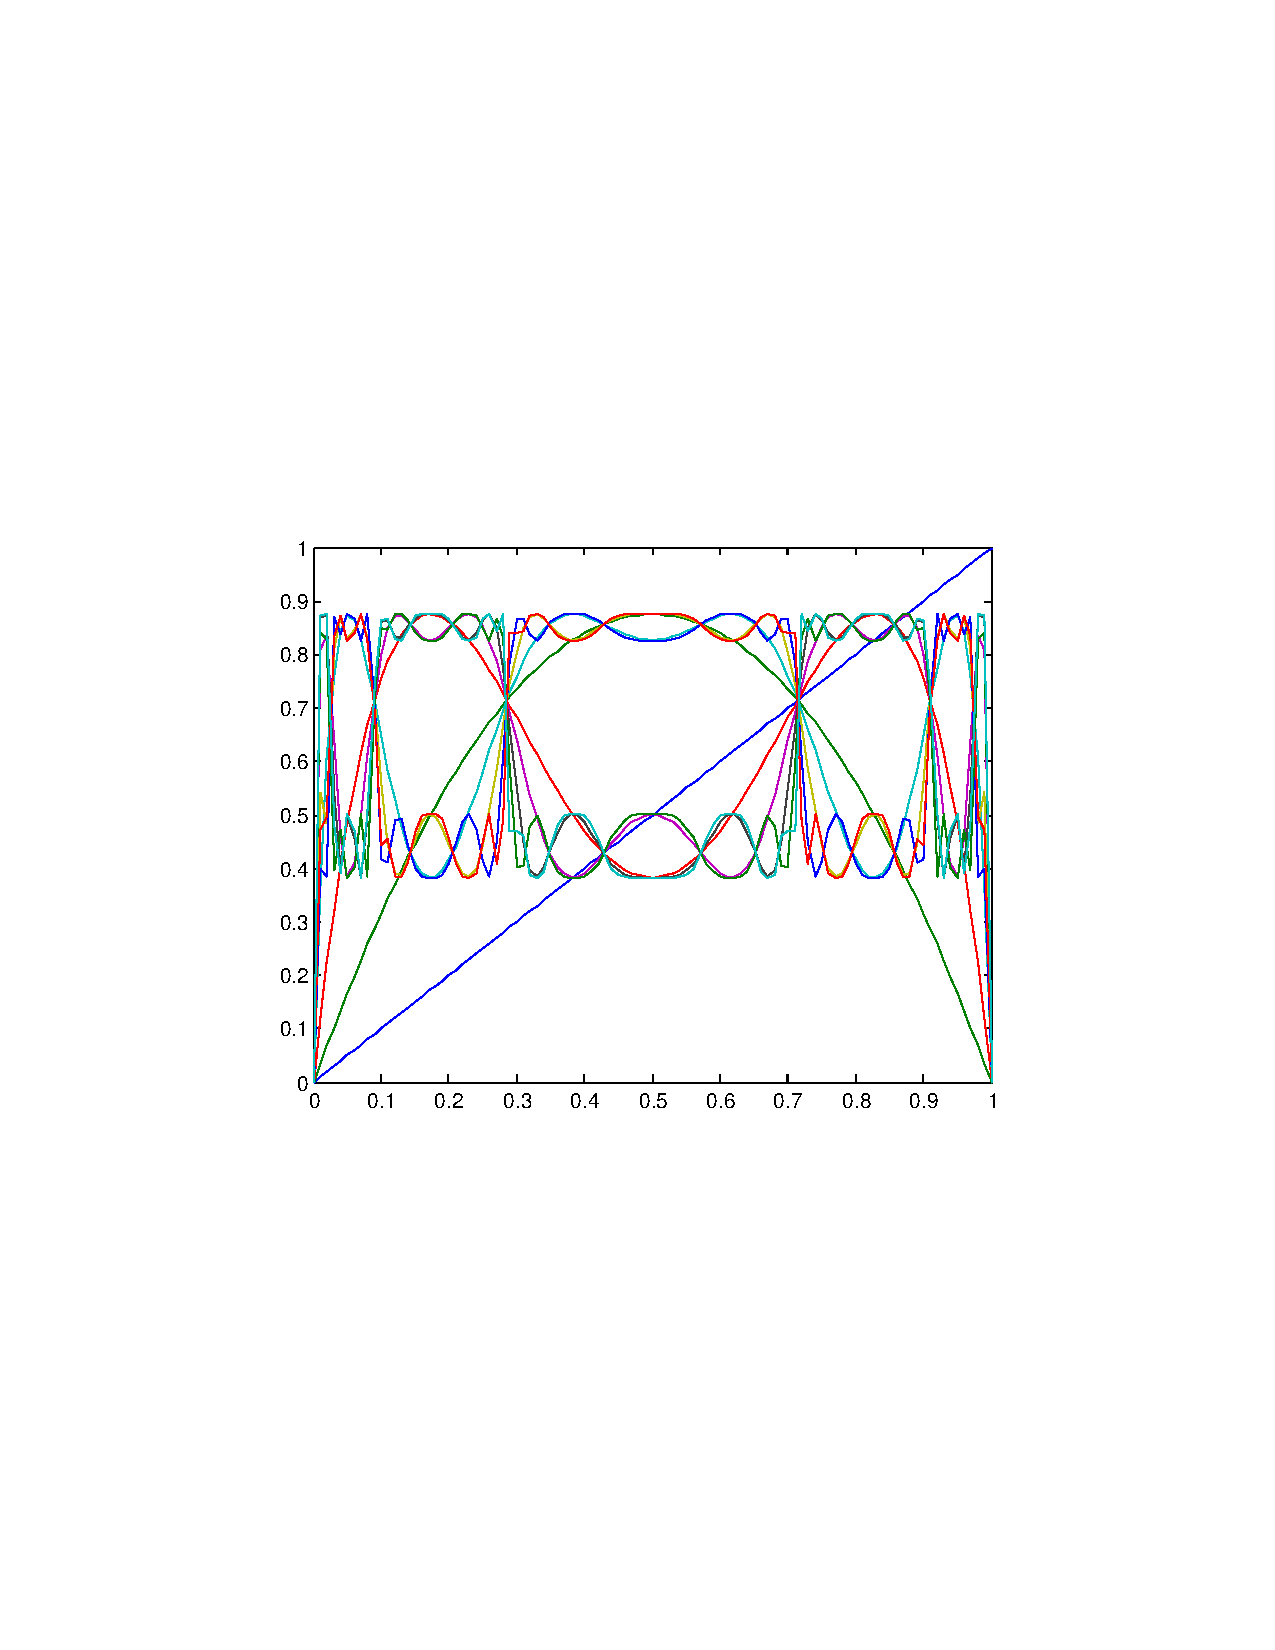
\includegraphics[width=\textwidth]{plot_iterates_3}
\end{center}
}



\end{document}